\documentclass{article}
\usepackage{color}
%% ODER: format ==         = "\mathrel{==}"
%% ODER: format /=         = "\neq "
%
%
\makeatletter
\@ifundefined{lhs2tex.lhs2tex.sty.read}%
  {\@namedef{lhs2tex.lhs2tex.sty.read}{}%
   \newcommand\SkipToFmtEnd{}%
   \newcommand\EndFmtInput{}%
   \long\def\SkipToFmtEnd#1\EndFmtInput{}%
  }\SkipToFmtEnd

\newcommand\ReadOnlyOnce[1]{\@ifundefined{#1}{\@namedef{#1}{}}\SkipToFmtEnd}
\usepackage{amstext}
\usepackage{amssymb}
\usepackage{stmaryrd}
\DeclareFontFamily{OT1}{cmtex}{}
\DeclareFontShape{OT1}{cmtex}{m}{n}
  {<5><6><7><8>cmtex8
   <9>cmtex9
   <10><10.95><12><14.4><17.28><20.74><24.88>cmtex10}{}
\DeclareFontShape{OT1}{cmtex}{m}{it}
  {<-> ssub * cmtt/m/it}{}
\newcommand{\texfamily}{\fontfamily{cmtex}\selectfont}
\DeclareFontShape{OT1}{cmtt}{bx}{n}
  {<5><6><7><8>cmtt8
   <9>cmbtt9
   <10><10.95><12><14.4><17.28><20.74><24.88>cmbtt10}{}
\DeclareFontShape{OT1}{cmtex}{bx}{n}
  {<-> ssub * cmtt/bx/n}{}
\newcommand{\tex}[1]{\text{\texfamily#1}}	% NEU

\newcommand{\Sp}{\hskip.33334em\relax}


\newcommand{\Conid}[1]{\mathit{#1}}
\newcommand{\Varid}[1]{\mathit{#1}}
\newcommand{\anonymous}{\kern0.06em \vbox{\hrule\@width.5em}}
\newcommand{\plus}{\mathbin{+\!\!\!+}}
\newcommand{\bind}{\mathbin{>\!\!\!>\mkern-6.7mu=}}
\newcommand{\rbind}{\mathbin{=\mkern-6.7mu<\!\!\!<}}% suggested by Neil Mitchell
\newcommand{\sequ}{\mathbin{>\!\!\!>}}
\renewcommand{\leq}{\leqslant}
\renewcommand{\geq}{\geqslant}
\usepackage{polytable}

%mathindent has to be defined
\@ifundefined{mathindent}%
  {\newdimen\mathindent\mathindent\leftmargini}%
  {}%

\def\resethooks{%
  \global\let\SaveRestoreHook\empty
  \global\let\ColumnHook\empty}
\newcommand*{\savecolumns}[1][default]%
  {\g@addto@macro\SaveRestoreHook{\savecolumns[#1]}}
\newcommand*{\restorecolumns}[1][default]%
  {\g@addto@macro\SaveRestoreHook{\restorecolumns[#1]}}
\newcommand*{\aligncolumn}[2]%
  {\g@addto@macro\ColumnHook{\column{#1}{#2}}}

\resethooks

\newcommand{\onelinecommentchars}{\quad-{}- }
\newcommand{\commentbeginchars}{\enskip\{-}
\newcommand{\commentendchars}{-\}\enskip}

\newcommand{\visiblecomments}{%
  \let\onelinecomment=\onelinecommentchars
  \let\commentbegin=\commentbeginchars
  \let\commentend=\commentendchars}

\newcommand{\invisiblecomments}{%
  \let\onelinecomment=\empty
  \let\commentbegin=\empty
  \let\commentend=\empty}

\visiblecomments

\newlength{\blanklineskip}
\setlength{\blanklineskip}{0.66084ex}

\newcommand{\hsindent}[1]{\quad}% default is fixed indentation
\let\hspre\empty
\let\hspost\empty
\newcommand{\NB}{\textbf{NB}}
\newcommand{\Todo}[1]{$\langle$\textbf{To do:}~#1$\rangle$}

\EndFmtInput
\makeatother
%
%
%
%
%
%
% This package provides two environments suitable to take the place
% of hscode, called "plainhscode" and "arrayhscode". 
%
% The plain environment surrounds each code block by vertical space,
% and it uses \abovedisplayskip and \belowdisplayskip to get spacing
% similar to formulas. Note that if these dimensions are changed,
% the spacing around displayed math formulas changes as well.
% All code is indented using \leftskip.
%
% Changed 19.08.2004 to reflect changes in colorcode. Should work with
% CodeGroup.sty.
%
\ReadOnlyOnce{polycode.fmt}%
\makeatletter

\newcommand{\hsnewpar}[1]%
  {{\parskip=0pt\parindent=0pt\par\vskip #1\noindent}}

% can be used, for instance, to redefine the code size, by setting the
% command to \small or something alike
\newcommand{\hscodestyle}{}

% The command \sethscode can be used to switch the code formatting
% behaviour by mapping the hscode environment in the subst directive
% to a new LaTeX environment.

\newcommand{\sethscode}[1]%
  {\expandafter\let\expandafter\hscode\csname #1\endcsname
   \expandafter\let\expandafter\endhscode\csname end#1\endcsname}

% "compatibility" mode restores the non-polycode.fmt layout.

\newenvironment{compathscode}%
  {\par\noindent
   \advance\leftskip\mathindent
   \hscodestyle
   \let\\=\@normalcr
   \let\hspre\(\let\hspost\)%
   \pboxed}%
  {\endpboxed\)%
   \par\noindent
   \ignorespacesafterend}

\newcommand{\compaths}{\sethscode{compathscode}}

% "plain" mode is the proposed default.
% It should now work with \centering.
% This required some changes. The old version
% is still available for reference as oldplainhscode.

\newenvironment{plainhscode}%
  {\hsnewpar\abovedisplayskip
   \advance\leftskip\mathindent
   \hscodestyle
   \let\hspre\(\let\hspost\)%
   \pboxed}%
  {\endpboxed%
   \hsnewpar\belowdisplayskip
   \ignorespacesafterend}

\newenvironment{oldplainhscode}%
  {\hsnewpar\abovedisplayskip
   \advance\leftskip\mathindent
   \hscodestyle
   \let\\=\@normalcr
   \(\pboxed}%
  {\endpboxed\)%
   \hsnewpar\belowdisplayskip
   \ignorespacesafterend}

% Here, we make plainhscode the default environment.

\newcommand{\plainhs}{\sethscode{plainhscode}}
\newcommand{\oldplainhs}{\sethscode{oldplainhscode}}
\plainhs

% The arrayhscode is like plain, but makes use of polytable's
% parray environment which disallows page breaks in code blocks.

\newenvironment{arrayhscode}%
  {\hsnewpar\abovedisplayskip
   \advance\leftskip\mathindent
   \hscodestyle
   \let\\=\@normalcr
   \(\parray}%
  {\endparray\)%
   \hsnewpar\belowdisplayskip
   \ignorespacesafterend}

\newcommand{\arrayhs}{\sethscode{arrayhscode}}

% The mathhscode environment also makes use of polytable's parray 
% environment. It is supposed to be used only inside math mode 
% (I used it to typeset the type rules in my thesis).

\newenvironment{mathhscode}%
  {\parray}{\endparray}

\newcommand{\mathhs}{\sethscode{mathhscode}}

% texths is similar to mathhs, but works in text mode.

\newenvironment{texthscode}%
  {\(\parray}{\endparray\)}

\newcommand{\texths}{\sethscode{texthscode}}

% The framed environment places code in a framed box.

\def\codeframewidth{\arrayrulewidth}
\RequirePackage{calc}

\newenvironment{framedhscode}%
  {\parskip=\abovedisplayskip\par\noindent
   \hscodestyle
   \arrayrulewidth=\codeframewidth
   \tabular{@{}|p{\linewidth-2\arraycolsep-2\arrayrulewidth-2pt}|@{}}%
   \hline\framedhslinecorrect\\{-1.5ex}%
   \let\endoflinesave=\\
   \let\\=\@normalcr
   \(\pboxed}%
  {\endpboxed\)%
   \framedhslinecorrect\endoflinesave{.5ex}\hline
   \endtabular
   \parskip=\belowdisplayskip\par\noindent
   \ignorespacesafterend}

\newcommand{\framedhslinecorrect}[2]%
  {#1[#2]}

\newcommand{\framedhs}{\sethscode{framedhscode}}

% The inlinehscode environment is an experimental environment
% that can be used to typeset displayed code inline.

\newenvironment{inlinehscode}%
  {\(\def\column##1##2{}%
   \let\>\undefined\let\<\undefined\let\\\undefined
   \newcommand\>[1][]{}\newcommand\<[1][]{}\newcommand\\[1][]{}%
   \def\fromto##1##2##3{##3}%
   \def\nextline{}}{\) }%

\newcommand{\inlinehs}{\sethscode{inlinehscode}}

% The joincode environment is a separate environment that
% can be used to surround and thereby connect multiple code
% blocks.

\newenvironment{joincode}%
  {\let\orighscode=\hscode
   \let\origendhscode=\endhscode
   \def\endhscode{\def\hscode{\endgroup\def\@currenvir{hscode}\\}\begingroup}
   %\let\SaveRestoreHook=\empty
   %\let\ColumnHook=\empty
   %\let\resethooks=\empty
   \orighscode\def\hscode{\endgroup\def\@currenvir{hscode}}}%
  {\origendhscode
   \global\let\hscode=\orighscode
   \global\let\endhscode=\origendhscode}%

\makeatother
\EndFmtInput
%
\usepackage{graphicx}

\definecolor{datatype}{RGB}{180,50,217}
\definecolor{constructor}{RGB}{145,55,200}
\definecolor{class}{RGB}{197,11,16}
\definecolor{fieldname}{RGB}{0,0,162}
\definecolor{prelude}{RGB}{64,80,117}
\definecolor{numeral}{RGB}{0,150,50}
\definecolor{infixoperator}{RGB}{42,0,217}
\definecolor{keyword}{RGB}{229,120,0}
\definecolor{special1}{RGB}{159,138,0}
\definecolor{string}{RGB}{150, 30, 30}
\definecolor{char}{RGB}{3, 106, 7}
\definecolor{constant}{RGB}{38, 139, 210}
\definecolor{function}{RGB}{50, 0, 250}

\newcommand{\lhsCHsyntax}[1]{\color{syntax}{{#1}}}
\newcommand{\lhsCHfunction}[1]{\color{function}{{#1}}}
\newcommand{\lhsCHinfixoperator}[1]{\color{infixoperator}{{#1}}}
\newcommand{\lhsCHprelude}[1]{\color{prelude}{\mathbf{#1}}}
\newcommand{\lhsCHkeyword}[1]{\color{keyword}{\textbf{#1}}}
\newcommand{\lhsCHconstructor}[1]{\color{constructor}{\textbf{#1}}}
\newcommand{\lhsCHtype}[1]{\color{datatype}{{#1}}}
\newcommand{\lhsCHclass}[1]{\color{class}{{#1}}}
\newcommand{\lhsCHconstant}[1]{\color{constant}{{#1}}}



%{-
%
% Copyright (C) 2012, Martin Varela
%
%    This program is free software; you can redistribute it and/or modify
%    it under the terms of the GNU General Public License as published by
%    the Free Software Foundation; either version 2 of the License, or
%    (at your option) any later version.
%
%    This program is distributed in the hope that it will be useful,
%    but WITHOUT ANY WARRANTY; without even the implied warranty of
%    MERCHANTABILITY or FITNESS FOR A PARTICULAR PURPOSE.  See the
%    GNU General Public License for more details.
%
%    You should have received a copy of the GNU General Public License along
%    with this program; if not, write to the Free Software Foundation, Inc.,
%    51 Franklin Street, Fifth Floor, Boston, MA 02110-1301 USA.
%
%-}

\begin{document}
\title{Gilbert Loss Trace Generator}
\author{ Mart\'\i n Varela - VTT}

\maketitle


\abstract{ This program allows the generation of several accurate (with respect
to pre--defined target values) loss traces following a simplified Gilbert loss
model (2-states, one with no losses, and one with loss probability = 1). For
subjective testing, the challenge lies in getting the right stats within a few
hundred packets, as test sequences are only $\sim 10s$ long. We take a
brute-force approach, generating several samples per combination of loss--rate
and mean loss burst size until enough  sufficiently good traces are generated.  }

\section{Preliminaries}

We will define our  $Main$ module and import some standard library functions and types.

\begin{hscode}\SaveRestoreHook
\column{B}{@{}>{\hspre}l<{\hspost}@{}}%
\column{E}{@{}>{\hspre}l<{\hspost}@{}}%
\>[B]{}\mathbf{module}\;\Conid{Main}\;\mathbf{where}{}\<[E]%
\\
\>[B]{}\mathbf{import}\;\Conid{\Conid{Data}.List}{}\<[E]%
\\
\>[B]{}\mathbf{import}\;\Conid{\Conid{System}.Random}{}\<[E]%
\\
\>[B]{}\mathbf{import}\;\Conid{\Conid{System}.Environment}{}\<[E]%
\ColumnHook
\end{hscode}\resethooks

\section{Packet Sequences}

A network flow is represented by a sequence of packets, which either arrive at 
their destination, or don't. We model this by the type $Packet$, defined as 
follows:

\begin{hscode}\SaveRestoreHook
\column{B}{@{}>{\hspre}l<{\hspost}@{}}%
\column{3}{@{}>{\hspre}l<{\hspost}@{}}%
\column{E}{@{}>{\hspre}l<{\hspost}@{}}%
\>[B]{}\mathbf{data}\; {\lhsCHtype{Packet}}\mathrel{=} {\lhsCHconstructor{P$_{\textbf{OK}}$}}\mid  {\lhsCHconstructor{P$_{\textbf{LOST}}$}}\;\mathbf{deriving}\; {\lhsCHclass{Eq}}{}\<[E]%
\\
\>[B]{}\mathbf{instance}\;\Conid{Show}\; {\lhsCHtype{Packet}}\;\mathbf{where}{}\<[E]%
\\
\>[B]{}\hsindent{3}{}\<[3]%
\>[3]{} {\lhsCHfunction{show}}\; {\lhsCHconstructor{P$_{\textbf{OK}}$}}\mathrel{=}\color{string}\text{\tt \char34 0\char34}{}\<[E]%
\\
\>[B]{}\hsindent{3}{}\<[3]%
\>[3]{} {\lhsCHfunction{show}}\; {\lhsCHconstructor{P$_{\textbf{LOST}}$}}\mathrel{=}\color{string}\text{\tt \char34 1\char34}{}\<[E]%
\ColumnHook
\end{hscode}\resethooks

\section{Valid Sequences}
\label{sec:valid}

 For a given sequence of packets $\sigma$, and target values for the loss rate
and mean loss burst size, $LR_{t}$ and $MLBS_{t}$ respectively, we consider
$\sigma$ to be suitable if the difference of the observed loss rate and MLBS in
the sequence, $LR_{\sigma}$ and $MLBS_{\sigma}$ and the target values is lower
than a given threshold.

We will define the thresholds at a $5\%$ of $LR_{t}$ for the loss rate, and 0.1
packets for the mean loss burst size., and so our conditions for accepting a 
sequence as valid are
$$
\mid LR_t - LR_{ \sigma }\mid \leq 0.05 \times LR_{t}
$$
and
$$
\mid MLBS_{t} - MLBS_{ \sigma }\mid \leq 0.1
$$

There is an issue when the definition of the mean loss burst size when no losses
occur. For some applications, it may be convenient to define it as 1, while in
other cases it might be better to define it as 0 (as indeed, if there are no
losses, speaking of the mean loss burst size does not make sense). However, for
QoE estimation purposes using PSQA or a similar technique, defining it as 0
might be problematic as it introduces a discontinuity in the mean loss burst
size axis (i.e. when there are losses, for any loss rate, the mean size of each
burst is at least 1). We will, therefore, define the mean loss burst size
of a lossless sequence as 1, define our functions accordingly.\\

We then have:
\begin{hscode}\SaveRestoreHook
\column{B}{@{}>{\hspre}l<{\hspost}@{}}%
\column{15}{@{}>{\hspre}l<{\hspost}@{}}%
\column{29}{@{}>{\hspre}l<{\hspost}@{}}%
\column{31}{@{}>{\hspre}l<{\hspost}@{}}%
\column{E}{@{}>{\hspre}l<{\hspost}@{}}%
\>[B]{} {\lhsCHfunction{checkSequence}}\mathbin{::} {\lhsCHtype{Double}}\to  {\lhsCHtype{Double}}\to [\mskip1.5mu  {\lhsCHtype{Packet}}\mskip1.5mu]\to  {\lhsCHtype{Bool}}{}\<[E]%
\\
\>[B]{} {\lhsCHfunction{checkSequence}}\;\Varid{tlr}\;\Varid{tmlbs}\;\Varid{s}{}\<[E]%
\\
\>[B]{}\hsindent{15}{}\<[15]%
\>[15]{}\mid \Varid{tlr} {\lhsCHinfixoperator{\ \mathbin{\textgreater}\ }}\color{numeral}{ 0 }{}\<[29]%
\>[29]{}\mathrel{=}(\Varid{abs} {\lhsCHinfixoperator{\ \mathbin{\ \mathbin{\$}\ }\ }}\Varid{tlr} {\lhsCHinfixoperator{\ \mathbin{-}\ }} {\lhsCHfunction{lr}}\;\Varid{s}) {\lhsCHinfixoperator{\ \mathbin{\ \leq\ }\ }}\color{numeral}{ 0.05 } {\lhsCHinfixoperator{\ \mathbin{*}\ }}\Varid{tlr} {\lhsCHinfixoperator{\ \mathbin{\ \mathrel{\wedge}\ }\ }}{}\<[E]%
\\
\>[29]{}\hsindent{2}{}\<[31]%
\>[31]{}(\Varid{abs} {\lhsCHinfixoperator{\ \mathbin{\ \mathbin{\$}\ }\ }}\Varid{tmlbs} {\lhsCHinfixoperator{\ \mathbin{-}\ }} {\lhsCHfunction{mlbs}}\;\Varid{s}) {\lhsCHinfixoperator{\ \mathbin{\ \leq\ }\ }}\color{numeral}{ 0.1 }{}\<[E]%
\\
\>[B]{}\hsindent{15}{}\<[15]%
\>[15]{}\mid \Varid{otherwise}{}\<[29]%
\>[29]{}\mathrel{=} {\lhsCHfunction{lr}}\;\Varid{s} {\lhsCHinfixoperator{\ \mathbin{\ \equiv\ }\ }}\color{numeral}{ 0 }{}\<[E]%
\ColumnHook
\end{hscode}\resethooks

We calculate the loss rate in the sequence by counting the number of lost
packets and dividing over the sequence length.  

\begin{hscode}\SaveRestoreHook
\column{B}{@{}>{\hspre}l<{\hspost}@{}}%
\column{8}{@{}>{\hspre}c<{\hspost}@{}}%
\column{8E}{@{}l@{}}%
\column{11}{@{}>{\hspre}l<{\hspost}@{}}%
\column{E}{@{}>{\hspre}l<{\hspost}@{}}%
\>[B]{} {\lhsCHfunction{lr}}\;\Varid{xs}{}\<[8]%
\>[8]{}\mathrel{=}{}\<[8E]%
\>[11]{}(\Varid{fromIntegral} {\lhsCHinfixoperator{\ \mathbin{.}\ }} {\lhsCHfunction{length}} {\lhsCHinfixoperator{\ \mathbin{.}\ }} {\lhsCHfunction{filter}}\;( {\lhsCHinfixoperator{\ \mathbin{\ \equiv\ }\ }} {\lhsCHconstructor{P$_{\textbf{LOST}}$}}) {\lhsCHinfixoperator{\ \mathbin{\ \mathbin{\$}\ }\ }}\Varid{xs}) {\lhsCHinfixoperator{\ \mathbin{/}\ }}{}\<[E]%
\\
\>[11]{}(\Varid{fromIntegral} {\lhsCHinfixoperator{\ \mathbin{.}\ }} {\lhsCHfunction{length}} {\lhsCHinfixoperator{\ \mathbin{\ \mathbin{\$}\ }\ }}\Varid{xs}){}\<[E]%
\ColumnHook
\end{hscode}\resethooks

The mean loss burst size is calculated as the average of the lengths of loss
events (i.e. instances where one or more packets are lost). To this end we
extract the loss events from the sequence, and calculate the average of their
lengths. As discussed above, if there are no losses, then we define the mean
loss burst size as one.

\begin{hscode}\SaveRestoreHook
\column{B}{@{}>{\hspre}l<{\hspost}@{}}%
\column{3}{@{}>{\hspre}l<{\hspost}@{}}%
\column{5}{@{}>{\hspre}l<{\hspost}@{}}%
\column{6}{@{}>{\hspre}c<{\hspost}@{}}%
\column{6E}{@{}l@{}}%
\column{9}{@{}>{\hspre}l<{\hspost}@{}}%
\column{15}{@{}>{\hspre}c<{\hspost}@{}}%
\column{15E}{@{}l@{}}%
\column{18}{@{}>{\hspre}l<{\hspost}@{}}%
\column{30}{@{}>{\hspre}c<{\hspost}@{}}%
\column{30E}{@{}l@{}}%
\column{33}{@{}>{\hspre}l<{\hspost}@{}}%
\column{E}{@{}>{\hspre}l<{\hspost}@{}}%
\>[B]{} {\lhsCHfunction{mlbs}}\;\Varid{xs}{}\<[E]%
\\
\>[B]{}\hsindent{6}{}\<[6]%
\>[6]{}\mid {}\<[6E]%
\>[9]{} {\lhsCHfunction{length}}\;\Varid{l\char95 events} {\lhsCHinfixoperator{\ \mathbin{\textgreater}\ }}\color{numeral}{ 0 }{}\<[30]%
\>[30]{}\mathrel{=}{}\<[30E]%
\>[33]{}(\Varid{fromIntegral} {\lhsCHinfixoperator{\ \mathbin{.}\ }}\Varid{sum} {\lhsCHinfixoperator{\ \mathbin{.}\ }} {\lhsCHfunction{map}}\; {\lhsCHfunction{length}} {\lhsCHinfixoperator{\ \mathbin{\ \mathbin{\$}\ }\ }}{}\<[E]%
\\
\>[33]{}\Varid{l\char95 events}) {\lhsCHinfixoperator{\ \mathbin{/}\ }}(\Varid{fromIntegral} {\lhsCHinfixoperator{\ \mathbin{.}\ }} {\lhsCHfunction{length}} {\lhsCHinfixoperator{\ \mathbin{\ \mathbin{\$}\ }\ }}{}\<[E]%
\\
\>[33]{}\Varid{l\char95 events}){}\<[E]%
\\
\>[B]{}\hsindent{6}{}\<[6]%
\>[6]{}\mid {}\<[6E]%
\>[9]{}\Varid{otherwise}{}\<[30]%
\>[30]{}\mathrel{=}{}\<[30E]%
\>[33]{}\color{numeral}{ 1 }{}\<[E]%
\\
\>[B]{}\hsindent{3}{}\<[3]%
\>[3]{}\mathbf{where}{}\<[E]%
\\
\>[3]{}\hsindent{2}{}\<[5]%
\>[5]{}\Varid{l\char95 events}{}\<[15]%
\>[15]{}\mathrel{=}{}\<[15E]%
\>[18]{}( {\lhsCHfunction{filter}}\;(\lambda \Varid{e}\to  {\lhsCHfunction{head}}\;\Varid{e} {\lhsCHinfixoperator{\ \mathbin{\ \equiv\ }\ }} {\lhsCHconstructor{P$_{\textbf{LOST}}$}})) {\lhsCHinfixoperator{\ \mathbin{.}\ }}{}\<[E]%
\\
\>[18]{}( {\lhsCHfunction{groupBy}}\;(\lambda \Varid{x}\;\Varid{y}\to \Varid{x} {\lhsCHinfixoperator{\ \mathbin{\ \equiv\ }\ }}\Varid{y} {\lhsCHinfixoperator{\ \mathbin{\ \mathrel{\wedge}\ }\ }}\Varid{y} {\lhsCHinfixoperator{\ \mathbin{\ \equiv\ }\ }} {\lhsCHconstructor{P$_{\textbf{LOST}}$}})) {\lhsCHinfixoperator{\ \mathbin{\ \mathbin{\$}\ }\ }}{}\<[E]%
\\
\>[18]{}\Varid{xs}{}\<[E]%
\ColumnHook
\end{hscode}\resethooks


\section{Sequence Generation}

In order to generate sequences with the desired loss process, we need to
calculate, from the target parameters $LR_t$ and $MLBS_t$, the probabilities for
the simplified Gilbert model. The conversion is given by
$$
 p = \frac{1}{MLBS_t}\frac{LR_t}{1-LR_t}
$$
and 
$$
q = \frac{1}{MLBS_t}
$$
where $p$ and $q$ correspond to the probabilities of going from the no--loss
state to the loss state, and vice--versa, respectively, as seen in Figure~\ref{fig:gilbert}.  

\begin{figure}[h]
\centering
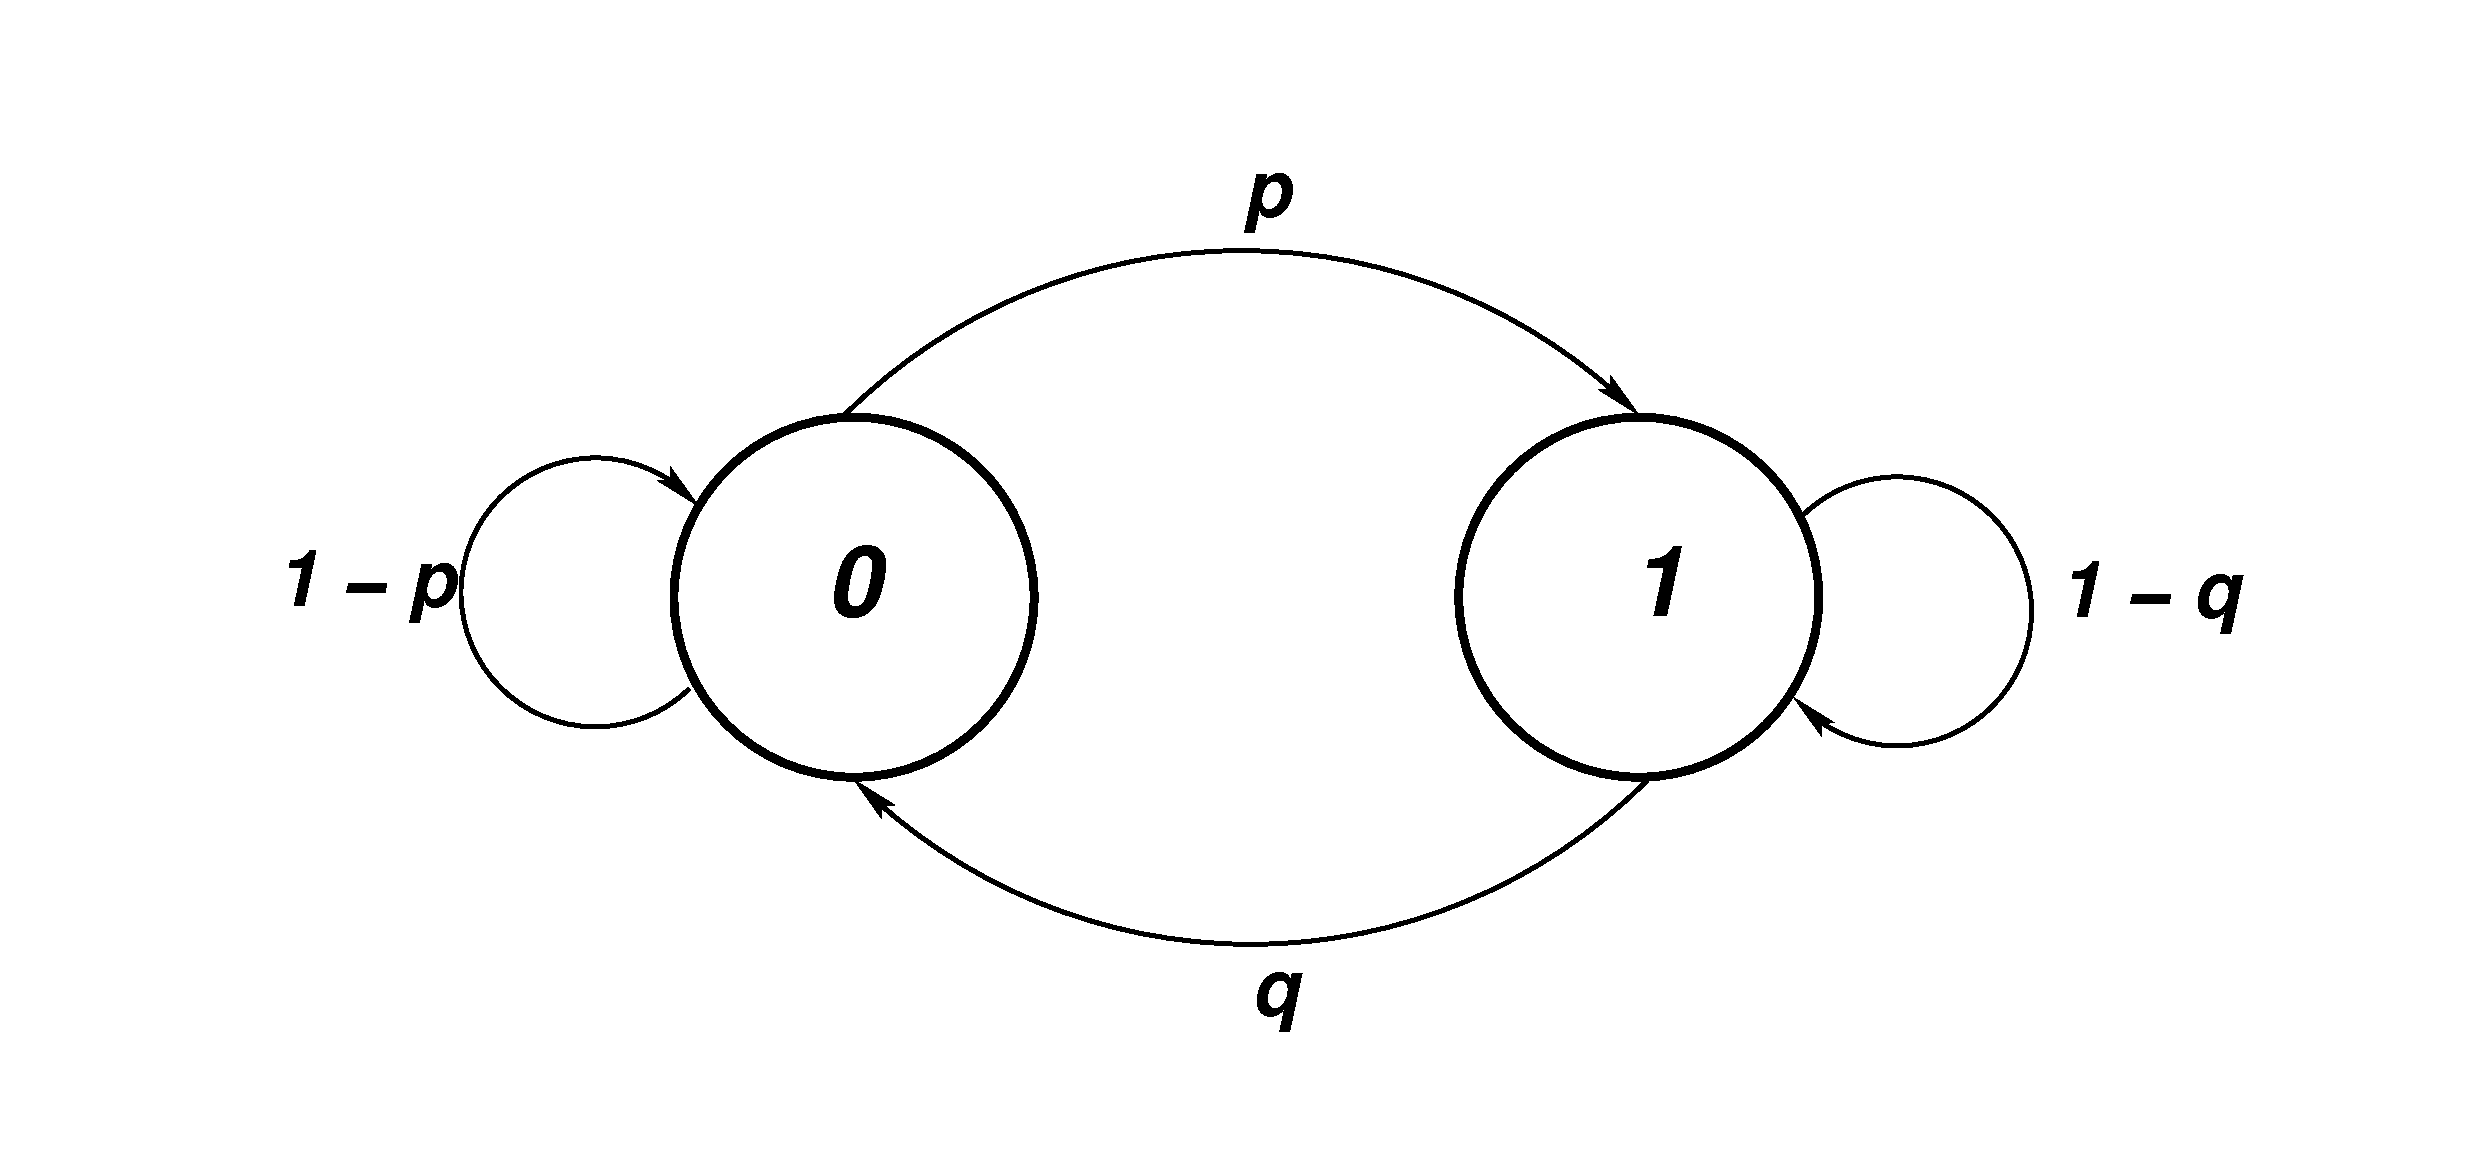
\includegraphics[scale=0.2]{figs/gilbert_simplified.pdf}
\caption{The simplified Gilbert model.}
\label{fig:gilbert}
\end{figure}


Sequences need to be generated with a pre--defined length, and we will need to
obtain several different sequences with similar statistical loss behavior. So if
we want to obtain $k$ sequences with a certain loss rate $tlr$ and mean loss
burst size $tmlbs$ within a certain tolerance as defined in
Section~\ref{sec:valid}, then we can imagine generating an infinite list of
sequences $ls$ with the target parameters and selecting from those the first $k$
sequences that are valid.

We can then write

\begin{hscode}\SaveRestoreHook
\column{B}{@{}>{\hspre}l<{\hspost}@{}}%
\column{21}{@{}>{\hspre}l<{\hspost}@{}}%
\column{33}{@{}>{\hspre}c<{\hspost}@{}}%
\column{33E}{@{}l@{}}%
\column{36}{@{}>{\hspre}l<{\hspost}@{}}%
\column{E}{@{}>{\hspre}l<{\hspost}@{}}%
\>[B]{} {\lhsCHfunction{selectSequences}}\mathbin{::}{}\<[21]%
\>[21]{} {\lhsCHtype{Int}}\to  {\lhsCHtype{Double}}\to  {\lhsCHtype{Double}}\to [\mskip1.5mu [\mskip1.5mu  {\lhsCHtype{Packet}}\mskip1.5mu]\mskip1.5mu]\to {}\<[E]%
\\
\>[21]{}[\mskip1.5mu [\mskip1.5mu  {\lhsCHtype{Packet}}\mskip1.5mu]\mskip1.5mu]{}\<[E]%
\\
\>[B]{} {\lhsCHfunction{selectSequences}}\;\Varid{k}\;\Varid{tlr}\;\Varid{tmlbs}\;\Varid{s}{}\<[33]%
\>[33]{}\mathrel{=}{}\<[33E]%
\>[36]{} {\lhsCHfunction{take}}\;\Varid{k} {\lhsCHinfixoperator{\ \mathbin{\ \mathbin{\$}\ }\ }}{}\<[E]%
\\
\>[36]{} {\lhsCHfunction{filter}}\;( {\lhsCHfunction{checkSequence}}\;\Varid{tlr}\;\Varid{tmlbs})\;\Varid{s}{}\<[E]%
\ColumnHook
\end{hscode}\resethooks

It now remains the task of generating the actual sequences with the desired
targets.  Since it would be useful to obtain repeatable traces, we start by
taking a seed as an argument. We'll use that seed to generate a pseudo--random
sequence of integer seeds for creating new generators for the actual packet loss
sequences.  In this way, we get the repeatability, and we keep a larger portion
of the code pure.

\begin{hscode}\SaveRestoreHook
\column{B}{@{}>{\hspre}l<{\hspost}@{}}%
\column{E}{@{}>{\hspre}l<{\hspost}@{}}%
\>[B]{} {\lhsCHfunction{seeds}}\;\Varid{s}\mathrel{=}(\Varid{randoms} {\lhsCHinfixoperator{\ \mathbin{\ \mathbin{\$}\ }\ }} {\lhsCHfunction{mkStdGen}}\;\Varid{s})\mathbin{::}[\mskip1.5mu  {\lhsCHtype{Int}}\mskip1.5mu]{}\<[E]%
\ColumnHook
\end{hscode}\resethooks

In order to generate the sequences, we need to implement the two--state Markov
chain depicted in Figure~\ref{fig:gilbert}. We use one of the previously
generated seeds to feed a new generator, and use this to simulate the chain.
So, the creation of a sequences takes as arguments the transition probabilities
for the Markov chain, the desired sequence length, and a seed for the
pseudo--random number generator. We always start from a loss--free state.

\begin{hscode}\SaveRestoreHook
\column{B}{@{}>{\hspre}l<{\hspost}@{}}%
\column{3}{@{}>{\hspre}l<{\hspost}@{}}%
\column{5}{@{}>{\hspre}l<{\hspost}@{}}%
\column{8}{@{}>{\hspre}l<{\hspost}@{}}%
\column{11}{@{}>{\hspre}l<{\hspost}@{}}%
\column{23}{@{}>{\hspre}l<{\hspost}@{}}%
\column{E}{@{}>{\hspre}l<{\hspost}@{}}%
\>[B]{} {\lhsCHfunction{createSequence}}\mathbin{::} {\lhsCHtype{Double}}\to  {\lhsCHtype{Double}}\to  {\lhsCHtype{Int}}\to  {\lhsCHtype{Int}}\to [\mskip1.5mu  {\lhsCHtype{Packet}}\mskip1.5mu]{}\<[E]%
\\
\>[B]{} {\lhsCHfunction{createSequence}}\;\Varid{tlr}\;\Varid{tmlbs}\;\Varid{k}\;\Varid{s}\mathrel{=} {\lhsCHfunction{unfoldr}}\;\Varid{fgen}\;(\Varid{p},\Varid{q}, {\lhsCHconstructor{P$_{\textbf{OK}}$}},\Varid{probs}){}\<[E]%
\\
\>[B]{}\hsindent{3}{}\<[3]%
\>[3]{}\mathbf{where}{}\<[E]%
\\
\>[3]{}\hsindent{2}{}\<[5]%
\>[5]{}\Varid{probs}\mathrel{=} {\lhsCHfunction{take}}\;\Varid{k} {\lhsCHinfixoperator{\ \mathbin{\ \mathbin{\$}\ }\ }}{}\<[23]%
\>[23]{}(\Varid{randoms} {\lhsCHinfixoperator{\ \mathbin{\ \mathbin{\$}\ }\ }} {\lhsCHfunction{mkStdGen}}\;\Varid{s})\mathbin{::}[\mskip1.5mu  {\lhsCHtype{Double}}\mskip1.5mu]{}\<[E]%
\\
\>[3]{}\hsindent{2}{}\<[5]%
\>[5]{}\Varid{p}{}\<[11]%
\>[11]{}\mathrel{=}(\Varid{tlr} {\lhsCHinfixoperator{\ \mathbin{/}\ }}(\color{numeral}{ 1 } {\lhsCHinfixoperator{\ \mathbin{-}\ }}\Varid{tlr})) {\lhsCHinfixoperator{\ \mathbin{/}\ }}\Varid{mbs}{}\<[E]%
\\
\>[3]{}\hsindent{2}{}\<[5]%
\>[5]{}\Varid{q}{}\<[11]%
\>[11]{}\mathrel{=}\color{numeral}{ 1 } {\lhsCHinfixoperator{\ \mathbin{/}\ }}\Varid{mbs}{}\<[E]%
\\
\>[3]{}\hsindent{2}{}\<[5]%
\>[5]{}\Varid{mbs}{}\<[E]%
\\
\>[5]{}\hsindent{3}{}\<[8]%
\>[8]{}\mid \Varid{tmlbs} {\lhsCHinfixoperator{\ \mathbin{\textgreater}\ }}\color{numeral}{ 0 }\mathrel{=}\Varid{tmlbs}{}\<[E]%
\\
\>[5]{}\hsindent{3}{}\<[8]%
\>[8]{}\mid \Varid{otherwise}\mathrel{=}\color{numeral}{ 1 }{}\<[E]%
\ColumnHook
\end{hscode}\resethooks
 
 \begin{hscode}\SaveRestoreHook
\column{B}{@{}>{\hspre}l<{\hspost}@{}}%
\column{3}{@{}>{\hspre}l<{\hspost}@{}}%
\column{5}{@{}>{\hspre}l<{\hspost}@{}}%
\column{7}{@{}>{\hspre}l<{\hspost}@{}}%
\column{10}{@{}>{\hspre}l<{\hspost}@{}}%
\column{12}{@{}>{\hspre}l<{\hspost}@{}}%
\column{15}{@{}>{\hspre}c<{\hspost}@{}}%
\column{15E}{@{}l@{}}%
\column{16}{@{}>{\hspre}l<{\hspost}@{}}%
\column{19}{@{}>{\hspre}l<{\hspost}@{}}%
\column{21}{@{}>{\hspre}l<{\hspost}@{}}%
\column{26}{@{}>{\hspre}l<{\hspost}@{}}%
\column{40}{@{}>{\hspre}c<{\hspost}@{}}%
\column{40E}{@{}l@{}}%
\column{43}{@{}>{\hspre}l<{\hspost}@{}}%
\column{E}{@{}>{\hspre}l<{\hspost}@{}}%
\>[B]{}\Varid{fgen}\mathbin{::}{}\<[10]%
\>[10]{}( {\lhsCHtype{Double}}, {\lhsCHtype{Double}}, {\lhsCHtype{Packet}},[\mskip1.5mu  {\lhsCHtype{Double}}\mskip1.5mu])\to {}\<[E]%
\\
\>[10]{}\Conid{Maybe}\;( {\lhsCHtype{Packet}},( {\lhsCHtype{Double}}, {\lhsCHtype{Double}}, {\lhsCHtype{Packet}},[\mskip1.5mu  {\lhsCHtype{Double}}\mskip1.5mu])){}\<[E]%
\\[\blanklineskip]%
\>[B]{}\Varid{fgen}\;{}\<[7]%
\>[7]{}(\anonymous ,{}\<[12]%
\>[12]{}\anonymous ,{}\<[16]%
\>[16]{}\anonymous ,{}\<[26]%
\>[26]{}[\mskip1.5mu \mskip1.5mu]){}\<[40]%
\>[40]{}\mathrel{=}{}\<[40E]%
\>[43]{}\Conid{Nothing}{}\<[E]%
\\
\>[B]{}\Varid{fgen}\;{}\<[7]%
\>[7]{}(\Varid{p},{}\<[12]%
\>[12]{}\Varid{q},{}\<[16]%
\>[16]{}\Varid{current},{}\<[26]%
\>[26]{}\Varid{probs}){}\<[40]%
\>[40]{}\mathrel{=}{}\<[40E]%
\>[43]{}\Conid{Just}\;(\Varid{next},(\Varid{p},\Varid{q},\Varid{next},\Varid{tail}\;\Varid{probs})){}\<[E]%
\\
\>[B]{}\hsindent{3}{}\<[3]%
\>[3]{}\mathbf{where}{}\<[E]%
\\
\>[3]{}\hsindent{2}{}\<[5]%
\>[5]{}\Varid{next}\mathrel{=}\mathbf{case}\;\Varid{current}\;\mathbf{of}{}\<[E]%
\\
\>[5]{}\hsindent{2}{}\<[7]%
\>[7]{} {\lhsCHconstructor{P$_{\textbf{OK}}$}}{}\<[15]%
\>[15]{}\to {}\<[15E]%
\>[19]{}\mathbf{if}\;(\Varid{p} {\lhsCHinfixoperator{\ \mathbin{\ \leq\ }\ }} {\lhsCHfunction{head}}\;\Varid{probs}){}\<[E]%
\\
\>[19]{}\hsindent{2}{}\<[21]%
\>[21]{}\mathbf{then}\; {\lhsCHconstructor{P$_{\textbf{OK}}$}}{}\<[E]%
\\
\>[19]{}\hsindent{2}{}\<[21]%
\>[21]{}\mathbf{else}\; {\lhsCHconstructor{P$_{\textbf{LOST}}$}}{}\<[E]%
\\
\>[5]{}\hsindent{2}{}\<[7]%
\>[7]{} {\lhsCHconstructor{P$_{\textbf{LOST}}$}}{}\<[15]%
\>[15]{}\to {}\<[15E]%
\>[19]{}\mathbf{if}\;(\Varid{q} {\lhsCHinfixoperator{\ \mathbin{\ \leq\ }\ }} {\lhsCHfunction{head}}\;\Varid{probs}){}\<[E]%
\\
\>[19]{}\hsindent{2}{}\<[21]%
\>[21]{}\mathbf{then}\; {\lhsCHconstructor{P$_{\textbf{LOST}}$}}{}\<[E]%
\\
\>[19]{}\hsindent{2}{}\<[21]%
\>[21]{}\mathbf{else}\; {\lhsCHconstructor{P$_{\textbf{OK}}$}}{}\<[E]%
\ColumnHook
\end{hscode}\resethooks

Having the means to generate sequences with the desired target loss
characteristics, we just create an infinite list of such sequences, from which
we will then choose as many as we need. It should be noted that depending on the
target values and tolerances, this might result in a non--halting computation,
as some combinations of target values and sequence length are not feasible.

\begin{hscode}\SaveRestoreHook
\column{B}{@{}>{\hspre}l<{\hspost}@{}}%
\column{26}{@{}>{\hspre}c<{\hspost}@{}}%
\column{26E}{@{}l@{}}%
\column{29}{@{}>{\hspre}l<{\hspost}@{}}%
\column{E}{@{}>{\hspre}l<{\hspost}@{}}%
\>[B]{} {\lhsCHfunction{sequences}}\mathbin{::} {\lhsCHtype{Double}}\to  {\lhsCHtype{Double}}\to  {\lhsCHtype{Int}}\to  {\lhsCHtype{Int}}\to [\mskip1.5mu [\mskip1.5mu  {\lhsCHtype{Packet}}\mskip1.5mu]\mskip1.5mu]{}\<[E]%
\\
\>[B]{} {\lhsCHfunction{sequences}}\;\Varid{tlr}\;\Varid{tmlbs}\;\Varid{k}\;\Varid{s}{}\<[26]%
\>[26]{}\mathrel{=}{}\<[26E]%
\>[29]{} {\lhsCHfunction{map}}\;( {\lhsCHfunction{createSequence}}\;\Varid{tlr}\;\Varid{tmlbs}\;\Varid{k}) {\lhsCHinfixoperator{\ \mathbin{\ \mathbin{\$}\ }\ }}{}\<[E]%
\\
\>[29]{} {\lhsCHfunction{seeds}}\;\Varid{s}{}\<[E]%
\ColumnHook
\end{hscode}\resethooks


With the sequence generation solved, we can now build the rest of the program,
which will take arguments for the target loss rate, the target mean loss burst
size, the length of the sequences to be generated, the number of sequences to be
generated, and a seed for the RNG. The program will then create a file per
sequence generated, and a file with the actual loss rates and mean loss burst 
sizes of the sequences generated, for validation purposes.

\begin{hscode}\SaveRestoreHook
\column{B}{@{}>{\hspre}l<{\hspost}@{}}%
\column{3}{@{}>{\hspre}l<{\hspost}@{}}%
\column{7}{@{}>{\hspre}l<{\hspost}@{}}%
\column{10}{@{}>{\hspre}l<{\hspost}@{}}%
\column{14}{@{}>{\hspre}c<{\hspost}@{}}%
\column{14E}{@{}l@{}}%
\column{17}{@{}>{\hspre}l<{\hspost}@{}}%
\column{21}{@{}>{\hspre}c<{\hspost}@{}}%
\column{21E}{@{}l@{}}%
\column{24}{@{}>{\hspre}l<{\hspost}@{}}%
\column{E}{@{}>{\hspre}l<{\hspost}@{}}%
\>[B]{}\Varid{main}\mathrel{=}\mathbf{do}{}\<[E]%
\\
\>[B]{}\hsindent{3}{}\<[3]%
\>[3]{}\Varid{args}\leftarrow \Varid{getArgs}{}\<[E]%
\\
\>[B]{}\hsindent{3}{}\<[3]%
\>[3]{}\mathbf{let}\;\Varid{tlr}{}\<[14]%
\>[14]{}\mathrel{=}{}\<[14E]%
\>[17]{}\Varid{read} {\lhsCHinfixoperator{\ \mathbin{\ \mathbin{\$}\ }\ }}\Varid{args} {\lhsCHinfixoperator{\ \mathbin{!!}\ }}\color{numeral}{ 0 }\mathbin{::} {\lhsCHtype{Double}}{}\<[E]%
\\
\>[3]{}\hsindent{4}{}\<[7]%
\>[7]{}\Varid{tmlbs}{}\<[14]%
\>[14]{}\mathrel{=}{}\<[14E]%
\>[17]{}\Varid{read} {\lhsCHinfixoperator{\ \mathbin{\ \mathbin{\$}\ }\ }}\Varid{args} {\lhsCHinfixoperator{\ \mathbin{!!}\ }}\color{numeral}{ 1 }\mathbin{::} {\lhsCHtype{Double}}{}\<[E]%
\\
\>[3]{}\hsindent{4}{}\<[7]%
\>[7]{}\Varid{lenS}{}\<[14]%
\>[14]{}\mathrel{=}{}\<[14E]%
\>[17]{}\Varid{read} {\lhsCHinfixoperator{\ \mathbin{\ \mathbin{\$}\ }\ }}\Varid{args} {\lhsCHinfixoperator{\ \mathbin{!!}\ }}\color{numeral}{ 2 }\mathbin{::} {\lhsCHtype{Int}}{}\<[E]%
\\
\>[3]{}\hsindent{4}{}\<[7]%
\>[7]{}\Varid{numS}{}\<[14]%
\>[14]{}\mathrel{=}{}\<[14E]%
\>[17]{}\Varid{read} {\lhsCHinfixoperator{\ \mathbin{\ \mathbin{\$}\ }\ }}\Varid{args} {\lhsCHinfixoperator{\ \mathbin{!!}\ }}\color{numeral}{ 3 }\mathbin{::} {\lhsCHtype{Int}}{}\<[E]%
\\
\>[3]{}\hsindent{4}{}\<[7]%
\>[7]{}\Varid{seed}{}\<[14]%
\>[14]{}\mathrel{=}{}\<[14E]%
\>[17]{}\Varid{read} {\lhsCHinfixoperator{\ \mathbin{\ \mathbin{\$}\ }\ }}\Varid{args} {\lhsCHinfixoperator{\ \mathbin{!!}\ }}\color{numeral}{ 4 }\mathbin{::} {\lhsCHtype{Int}}{}\<[E]%
\\
\>[B]{}\hsindent{3}{}\<[3]%
\>[3]{} {\lhsCHfunction{mapM}}\;{}\<[10]%
\>[10]{}( {\lhsCHfunction{createFile}}\;\Varid{tlr}\;\Varid{tmlbs}\;\Varid{seed}) {\lhsCHinfixoperator{\ \mathbin{\ \mathbin{\$}\ }\ }}{}\<[E]%
\\
\>[10]{} {\lhsCHfunction{zip}}\;[\mskip1.5mu \color{numeral}{ 1 }\mathinner{\ldotp\ldotp}\mskip1.5mu]\;{}\<[21]%
\>[21]{}({}\<[21E]%
\>[24]{} {\lhsCHfunction{selectSequences}}\;\Varid{numS}\;\Varid{tlr}\;\Varid{tmlbs} {\lhsCHinfixoperator{\ \mathbin{\ \mathbin{\$}\ }\ }}{}\<[E]%
\\
\>[24]{} {\lhsCHfunction{sequences}}\;\Varid{tlr}\;\Varid{tmlbs}\;\Varid{lenS}\;\Varid{seed}){}\<[E]%
\ColumnHook
\end{hscode}\resethooks

The creation of the trace and statistics files is handled like so:

\begin{hscode}\SaveRestoreHook
\column{B}{@{}>{\hspre}l<{\hspost}@{}}%
\column{3}{@{}>{\hspre}l<{\hspost}@{}}%
\column{7}{@{}>{\hspre}l<{\hspost}@{}}%
\column{16}{@{}>{\hspre}l<{\hspost}@{}}%
\column{17}{@{}>{\hspre}l<{\hspost}@{}}%
\column{27}{@{}>{\hspre}l<{\hspost}@{}}%
\column{28}{@{}>{\hspre}l<{\hspost}@{}}%
\column{E}{@{}>{\hspre}l<{\hspost}@{}}%
\>[B]{} {\lhsCHfunction{createFile}}\mathbin{::}{}\<[16]%
\>[16]{} {\lhsCHtype{Double}}\to  {\lhsCHtype{Double}}\to  {\lhsCHtype{Int}}\to {}\<[E]%
\\
\>[16]{}( {\lhsCHtype{Int}},[\mskip1.5mu  {\lhsCHtype{Packet}}\mskip1.5mu])\to \Conid{IO}\;(){}\<[E]%
\\[\blanklineskip]%
\>[B]{} {\lhsCHfunction{createFile}}\;\Varid{tlr}\;\Varid{tmlbs}\;\Varid{seed}\;(\Varid{seqno},\Varid{s})\mathrel{=}\mathbf{do}{}\<[E]%
\\
\>[B]{}\hsindent{3}{}\<[3]%
\>[3]{}\mathbf{let}\;\Varid{outfile}{}\<[17]%
\>[17]{}\mathrel{=}\Varid{concat}\;[\mskip1.5mu \color{string}\text{\tt \char34 trace\char95 \char34}{}\<[E]%
\\
\>[17]{}\hsindent{10}{}\<[27]%
\>[27]{}, {\lhsCHfunction{show}}\;\Varid{tlr}{}\<[E]%
\\
\>[17]{}\hsindent{10}{}\<[27]%
\>[27]{},\color{string}\text{\tt \char34 \char95 \char34}{}\<[E]%
\\
\>[17]{}\hsindent{10}{}\<[27]%
\>[27]{}, {\lhsCHfunction{show}}\;\Varid{tmlbs}{}\<[E]%
\\
\>[17]{}\hsindent{10}{}\<[27]%
\>[27]{},\color{string}\text{\tt \char34 \char95 \char34}{}\<[E]%
\\
\>[17]{}\hsindent{10}{}\<[27]%
\>[27]{}, {\lhsCHfunction{show}}\;\Varid{seed}{}\<[E]%
\\
\>[17]{}\hsindent{10}{}\<[27]%
\>[27]{},\color{string}\text{\tt \char34 \char95 \char34}{}\<[E]%
\\
\>[17]{}\hsindent{10}{}\<[27]%
\>[27]{}, {\lhsCHfunction{show}}\;\Varid{seqno}{}\<[E]%
\\
\>[17]{}\hsindent{10}{}\<[27]%
\>[27]{},\color{string}\text{\tt \char34 .txt\char34}\mskip1.5mu]{}\<[E]%
\\
\>[3]{}\hsindent{4}{}\<[7]%
\>[7]{}\Varid{statsfile}\mathrel{=}\Varid{concat}\;[\mskip1.5mu \color{string}\text{\tt \char34 stats\char95 \char34}{}\<[E]%
\\
\>[7]{}\hsindent{20}{}\<[27]%
\>[27]{}, {\lhsCHfunction{show}}\;\Varid{tlr}{}\<[E]%
\\
\>[7]{}\hsindent{20}{}\<[27]%
\>[27]{},\color{string}\text{\tt \char34 \char95 \char34}{}\<[E]%
\\
\>[7]{}\hsindent{20}{}\<[27]%
\>[27]{}, {\lhsCHfunction{show}}\;\Varid{tmlbs}{}\<[E]%
\\
\>[7]{}\hsindent{20}{}\<[27]%
\>[27]{},\color{string}\text{\tt \char34 \char95 \char34}{}\<[E]%
\\
\>[7]{}\hsindent{20}{}\<[27]%
\>[27]{}, {\lhsCHfunction{show}}\;\Varid{seed}{}\<[E]%
\\
\>[27]{}\hsindent{1}{}\<[28]%
\>[28]{},\color{string}\text{\tt \char34 .txt\char34}\mskip1.5mu]{}\<[E]%
\\
\>[3]{}\hsindent{4}{}\<[7]%
\>[7]{}\Varid{stats}{}\<[17]%
\>[17]{}\mathrel{=}\Varid{concat}\;[\mskip1.5mu \color{string}\text{\tt \char34 Sequence~\char34}{}\<[E]%
\\
\>[17]{}\hsindent{10}{}\<[27]%
\>[27]{}, {\lhsCHfunction{show}}\;\Varid{seqno}{}\<[E]%
\\
\>[17]{}\hsindent{10}{}\<[27]%
\>[27]{},\color{string}\text{\tt \char34 ~lr~=~\char34}{}\<[E]%
\\
\>[17]{}\hsindent{10}{}\<[27]%
\>[27]{}, {\lhsCHfunction{show}} {\lhsCHinfixoperator{\ \mathbin{\ \mathbin{\$}\ }\ }} {\lhsCHfunction{lr}}\;\Varid{s}{}\<[E]%
\\
\>[17]{}\hsindent{10}{}\<[27]%
\>[27]{},\color{string}\text{\tt \char34 ,~mlbs~=~\char34}{}\<[E]%
\\
\>[17]{}\hsindent{10}{}\<[27]%
\>[27]{}, {\lhsCHfunction{show}} {\lhsCHinfixoperator{\ \mathbin{\ \mathbin{\$}\ }\ }} {\lhsCHfunction{mlbs}}\;\Varid{s}{}\<[E]%
\\
\>[17]{}\hsindent{10}{}\<[27]%
\>[27]{},\color{string}\text{\tt \char34 \char92 n\char34}\mskip1.5mu]{}\<[E]%
\\[\blanklineskip]%
\>[B]{}\hsindent{3}{}\<[3]%
\>[3]{}\Varid{writeFile}\;\Varid{outfile} {\lhsCHinfixoperator{\ \mathbin{\ \mathbin{\$}\ }\ }}\Varid{concat} {\lhsCHinfixoperator{\ \mathbin{\ \mathbin{\$}\ }\ }} {\lhsCHfunction{map}}\;( {\lhsCHfunction{show}})\;\Varid{s}{}\<[E]%
\\
\>[B]{}\hsindent{3}{}\<[3]%
\>[3]{}\Varid{appendFile}\;\Varid{statsfile}\;\Varid{stats}{}\<[E]%
\ColumnHook
\end{hscode}\resethooks

\newpage
\section{License}

 Copyright (C) 2012, Mart\'\i n Varela

    This program is free software; you can redistribute it and/or modify
    it under the terms of the GNU General Public License as published by
    the Free Software Foundation; either version 2 of the License, or
    (at your option) any later version.

    This program is distributed in the hope that it will be useful,
    but WITHOUT ANY WARRANTY; without even the implied warranty of
    MERCHANTABILITY or FITNESS FOR A PARTICULAR PURPOSE.  See the
    GNU General Public License for more details.

    You should have received a copy of the GNU General Public License along
    with this program; if not, write to the Free Software Foundation, Inc.,
    51 Franklin Street, Fifth Floor, Boston, MA 02110-1301 USA.


\end{document}
